\section{Challenges and Opportunities}\label{sec:challenges}

Data access can become challenging in PHYSLITE when branches with custom objects need to be read or when full systematics need to be handled.
As columnar analysis processes events in batches, this requires that the ATLAS Combined Performance (CP) tools and algorithms that handle these challenges must also be able to operate on data in batches and have the appropriate interfaces.
The current Run 3 model for CP tools is to operate on the ATLAS xAOD event data model (EDM) for all the calculations per event and then to write the systematics to disk for future access~\cite{SOFT-2022-02}.
This process is I/O intensive and computationally inefficient, but has excellent physics performance and configurability for the current ATLAS analysis model.
As a data access layer the xAOD interface also makes assumptions about the underlying I/O layer, memory model, and processing environment, which do not match well to the expectations of columnar frameworks.
The challenge for a fully columnar CP tool framework is to adapt to the on-the-fly computation of the columnar paradigm --- furthering the ``trade disk for compute'' strategy --- while still being performant enough to not be a bottleneck.

The refactoring process for columnar tools in the ATLAS Analysis Model Group (AMG) has also offered design improvement opportunities to create more Pythonic end-user APIs for the ATLAS CP tools.
As seen in~\Cref{fig:columnar_cp_tools_diagram}, creating Pythonic APIs for users allows for integration with the broader scientific Python ecosystem, and through efficient binding layers all data can be passed through to the \texttt{C++} CP tools for efficient computation, and then the results can be exposed to the users again.
By using the \texttt{nanobind}~\cite{nanobind} \texttt{C++}-to-Python bindings library it becomes possible to have zero-copy operations to and from $n$-dimensional array libraries in Python, including those which support hardware accelerators like GPUs, and full design control of the high-level user API.
The API design ability is quite powerful, as it allows for unification of interfaces to CP tools without requiring individual CP tools to redesign their \texttt{C++} APIs.

\begin{figure}
    \centering
    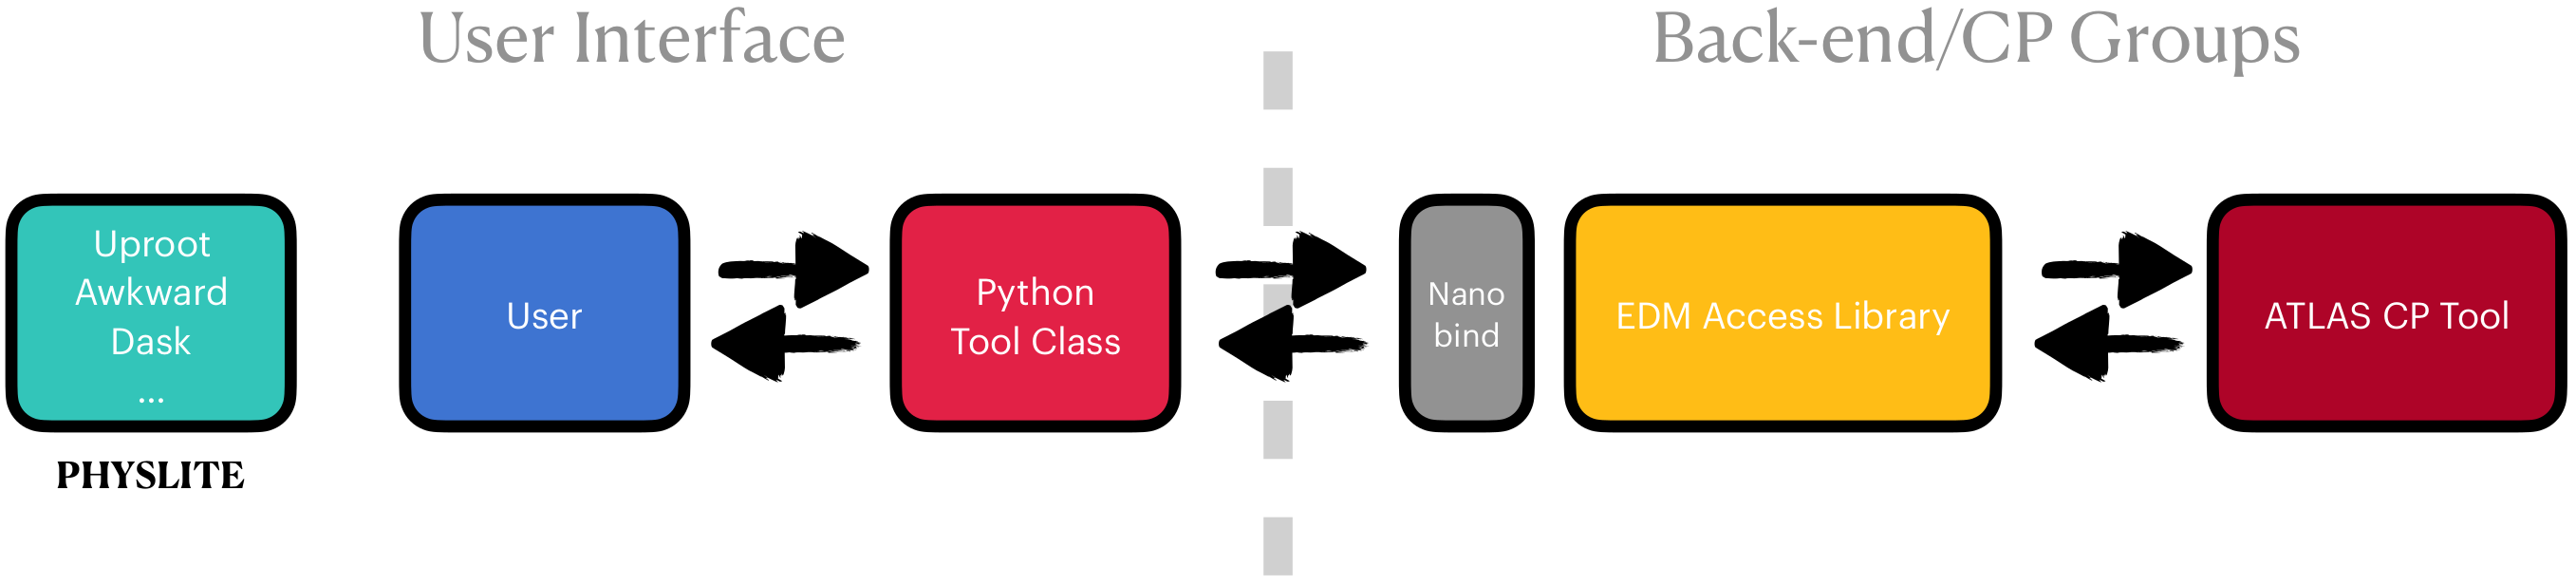
\includegraphics[width=\textwidth]{columnar_cp_tools_diagram.png}
    \caption{Cartoon of the data interface layers for the Pythonic interface to the columnar CP tools~\cite{Vigl:ACAT_2024}.
The user is presented with a high-level Pythonic API for operating on columns of PHYSLITE data (e.g. as NumPy or Awkward arrays) that has a similar design to common Python array libraries.
Through \texttt{nanobind} zero-copy buffers, the data columns are passed directly to the performant \texttt{C++} columnar CP tools for computation, and the results are returned to the user level as transformed arrays.}
    \label{fig:columnar_cp_tools_diagram}
\end{figure}
